
\documentclass[12pt]{standalone}
\usepackage{tikz}
\usetikzlibrary{automata,positioning}
\begin{document}
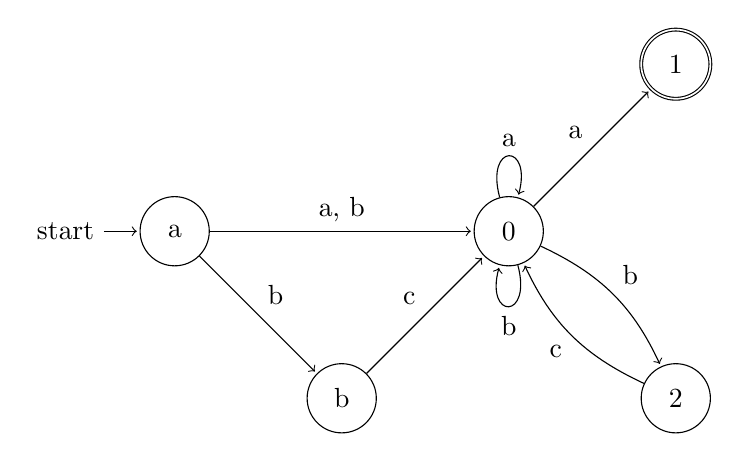
\begin{tikzpicture}[shorten >=1pt,node distance=3cm,on grid,auto] 
    \node[state, initial] (21)    {a};
    \node[state] (22) [below right=of 21] {b};
   \node[state] (0) [above right= of 22]   {$0$}; 
   \node[state,accepting] (1) [above right=of 0] {$1$}; 
   \node[state] (2) [below right=of 0] {$2$};

    \path[->] (21) edge node  {a, b} (0);
    \path[->] (21) edge node  {b} (22);
    \path[->] (22) edge node  {c} (0);
    \path[->] (0) edge [loop above] node  {a} (0);
    \path[->] (0) edge [loop below] node  {b} (0);
    \path[->] (0) edge  node {a} (1);
    \path[->] (0) edge [bend left = 20]  node {b} (2);
    \path[->] (2) edge [bend left = 20]  node {c} (0);
\end{tikzpicture}
\end{document}  

